\section{Signal Systematics}
\label{sec:signalsys}
We consider a variety of systematic uncertainties on the signal efficiency and distribution. Some are common to more 
inclusive SUSY analyses~\cite{RA2b:Moriond} and there are additional systematics related to $b\bar{b}$ tagging efficiency and 
the effect of the pruned mass scale and resolution on the signal efficiency.  
\begin{itemize}
\item {\bf Luminosity:} The recommendation for the 2016 dataset is currently a flat uncertainty of 2.5\%.
\item {\bf Isolated track veto:} A flat uncertainty of 2\% is assigned to the signal samples to account for any data/MC differences based on the study from the 2015 analysis~\cite{RA2b:Moriond}.
\item {\bf MC statistics:} The signal MC sample statistical uncertainty is generally 2-4\% .
\item {\bf Trigger efficiency:} The effect of the uncertainty on the signal yield is about 2\%.
\item {\bf Pileup reweighting:} The sensitivity to the pileup distribution was studied for various benchmark signal models by comparing events with $n_{\textrm{vtx}} < 20$ (low PU) or $n_{\textrm{vtx}} \geq 20$ (high PU). Accordingly, no pileup reweighting is applied to the signal MC samples and no associated uncertainty is assessed.
\item {\bf ISR:} An ISR correction is derived from tt events, with a selection requiring two lep-
tons (electrons or muons) and two b-tagged jets, implying that any other jets in the
event arise from ISR. The correction factors are 1.000, 0.920, 0.821, 0.715, 0.662, 0.561,
0.511 for NISR = 0, 1, 2, 3, 4, 5, 6+. The corrections are applied to the simulated signal jet
samples with an additional normalization factor, typically ∼1.15 (depending on the signal model), to ensure the overall cross section of the sample remains constant. The systematic uncertainty in these corrections is chosen to be half of the deviation from unity for each correction factor. The effect on the yield ranges from $0.0–1\%$, with the largest effect at high MET.
\item {\bf Scales:} The uncertainty is calculated using the envelope of the weights from varying the renormalization and factorization scales, $\mu_{R}$ and $\mu_{F}$,by a factor of 2 \cite{Cacciari:2003fi,Catani:2003zt}. The effect on the yield of is less than 0.1\%.
\item {\bf Jet Energy Corrections:} The jet energy corrections (JECs) are varied using the $p_{T}$-
and $\eta$-dependent jet energy scale uncertainties from the official database.
These variations are propagated into the various jet-dependent variables, including: HT, MET, $\Delta\phi(\textrm{MET},j_{i})$.
The overall effect is less than 1\%.
\item {\bf Jet Energy Resolution:} The jet momenta in the MC samples are smeared to match the jet energy resolution in data. The smearing factors are varied according to the uncertainties on the jet energy resolution measurements.
These variations are propagated into the various jet-dependent variables, including: HT, MET, $\Delta\phi(\textrm{MET},j_{i})$.
The overall effect ranges from 0.01\%.
\item {\bf PDFs:} The LHC4PDF prescription for the uncertainty on the total cross section is included as $\pm 1$ sigma bands in the results plots. No
additional uncertainty is considered for the uncertainty in the acceptance due to PDFs, as per SUSY group recommendation.
\end{itemize}
The above signal systematics are applied as an uncertainty on the signal normalization. These uncertainties are in general small. The main signal systematics 
come from the AK8 Jet Double-b tagging efficiency data/MC scale factors and the uncertainty on the pruned mass resolution.
The AK8 Jet Double-b tagging efficiency has an uncertainty which is propagated to the signal efficiency. This uncertainty is applied 
as a shape uncertainty across the Higgs tag regions and the anti-tag region. Also the pruned jet mass scale and resolution uncertainties are 
propogated to the final signal efficiency using POG recommendations. The pruned mass scale factor is derived using W-jets in semi-leptonic \ttbar and extrapolating to the H mass. This uncertainty is assigned a shape uncertainty on the signal mass window and the sideband. \\
\begin{itemize}
\item A data/MC scale-factor is derived from double-muon tag data selected with HLT Trigger \texttt{HLT\_BTagMu\_AK8Jet300\_Mu5\_v} and muon enriched QCD Monte-Carlo. The scale factors have mainly a statistical error along with a smaller set of systematic errors due to shape systematics, Jet-Energy scale uncertainty, Pile-up corrections, uncertainty on the number of tracks, uncertainty of b-fragmentation and  c-fragmentation, and the uncertainty on $K_{s}$ and $\Lambda$ fraction. 
\item The pruned mass scale-factor is derived by comparing the efficiency to select W-jets in data and MC within a mass window of $\left[65,85\right]$ GeV.  The fit for the gaussian resolution of the W-mass peak is shown in Figure~\ref{fig:WMassPeak} and the fit results are shown in Table~\ref{tab:WMassFit}. The mass scale between MC and data is consistent though MC predicts a narrower mass resolution compared to data. The jet mass in each event is smeared to mimic the pruned jet mass resolution in data and an uncertainty is assigned based on the ratio of efficiencies between the smeared and un-smeared cases. ~\cite{CMS_AN_2016-215}
\end{itemize} 

The summary of the signal systematics and their effect on the signal yields is shown in Table~\ref{tab:SignalSystSummary}. The dominant effect is from the mass resolution uncertainty.
%\item The pruned mass scale-factor is found to be consistent with 1.0 for the pruned mass-scale with an uncertainty based on the Jet-Energy scale uncertainty: $\sqrt{JES^2 + 0.02^2}$. The pruned jet mass-resolution scale-factor is found to $7\%$ with an uncertainty of $\sqrt{JER^2+0.103^2}$


\begin{figure}[htbp!]
  \begin{center}
    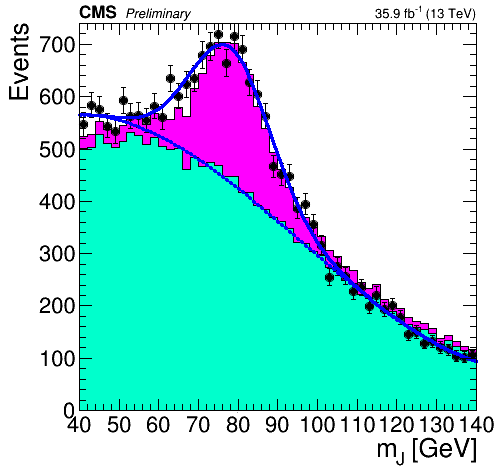
\includegraphics[width=0.48\linewidth]{figs/WMassPeakDataMC.png}

\end{center}
\caption{Pruned jet mass in in semi-leptonic \ttbar events. The mass peak for the W-jets is used to derive the mass resolution uncertainty. }
\label{fig:WMassPeak}
\end{figure}
\begin{table}[htbp!]
\centering
\begin{tabular}{c|c}
\hline \hline
\multicolumn{2}{c}{Data}\\
\hline \hline 
Mean &  $78.2 \pm 0.46$\\ \hline
Sigma & $10.10  \pm 0.671$ \\ \hline
\hline
\multicolumn{2}{c}{\ttbar MC}\\ \hline
\hline
Mean &  $ 78.4  \pm 0.35$\\ \hline
Sigma & $ 7.23   \pm 0.48$ \\ \hline
\end{tabular}
\caption{Fit results for W-mass resolution in data and MC}
\label{tab:WMassFit}
\end{table}

\begin{table}[htbp!]
\centering
\begin{tabular}{c|c}
\hline \hline
\multicolumn{2}{c}{Unc. on Normalization} \\  \hline
\hline \hline
Systematic & \% Effect on yields\\ \hline
Luminosity & 2.6\% \\ \hline
Trigger Eff. & 2.0\% \\ \hline
Iso. Track Veto & 2\%\\ \hline
ISR modeling & 0.01\% \\ \hline
PDF Scale & 0.1\% \\ \hline
JEC & 1\% \\ \hline
JER & 0.01\% \\ \hline
MC Stat & 1-4\% \\ \hline
\multicolumn{2}{c}{Shape Unc.} \\  \hline
Double-b SF & 6\% \\ \hline
Mass Resolution &1-15\% \\ \hline
\hline
\end{tabular}
\caption{
    Summary of signal shape and normalization uncertainties. 
}
\label{tab:SignalSystSummary}
\end{table}

